\chapter{Arhitektura i dizajn sustava}
		
		\textbf{\textit{dio 1. revizije}}\\

		Opis...

	
				
		\section{Baza podataka}
			
			\textbf{\textit{dio 1. revizije}}\\
			
		Opis baze...
		
			\subsection{Opis tablica}
			
				%Svjetlozelenom bojom označite primarni ključ. Svjetlo plavom označite strani ključ
				
				\begin{longtblr}[
					label=none,
					entry=none
					]{
						width = \textwidth,
						colspec={|X[6,l]|X[6, l]|X[20, l]|}, 
						rowhead = 1,
					} %definicija širine tablice, širine stupaca, poravnanje i broja redaka naslova tablice
					\hline \SetCell[c=3]{c}{\textbf{korisnik - ime tablice}}	 \\ \hline[3pt]
					\SetCell{LightGreen}$<$Ime varijable$>$ & $<$Tip varijable$>$	&  $<$IOpis varijable$>$	\\ \hline
						&  &   	\\ \hline 
					\SetCell{LightBlue}	&  &   	\\ \hline 
				\end{longtblr}
				
				
			
			\subsection{Dijagram baze podataka}
				
				%unos slike
				\begin{figure}[H]
					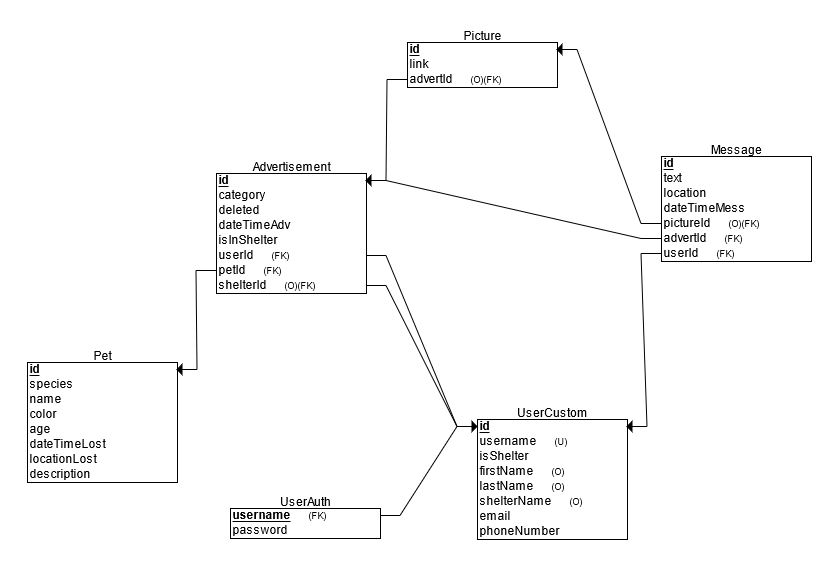
\includegraphics[scale=0.63]{dijagrami/dijagramBaze/relacijskiModel.PNG} %veličina slike u odnosu na originalnu datoteku i pozicija slike
					\centering
					\caption{Relacijski dijagram baze podataka}
					\label{fig:relDijagram}
				\end{figure}

				\begin{figure}[H]
					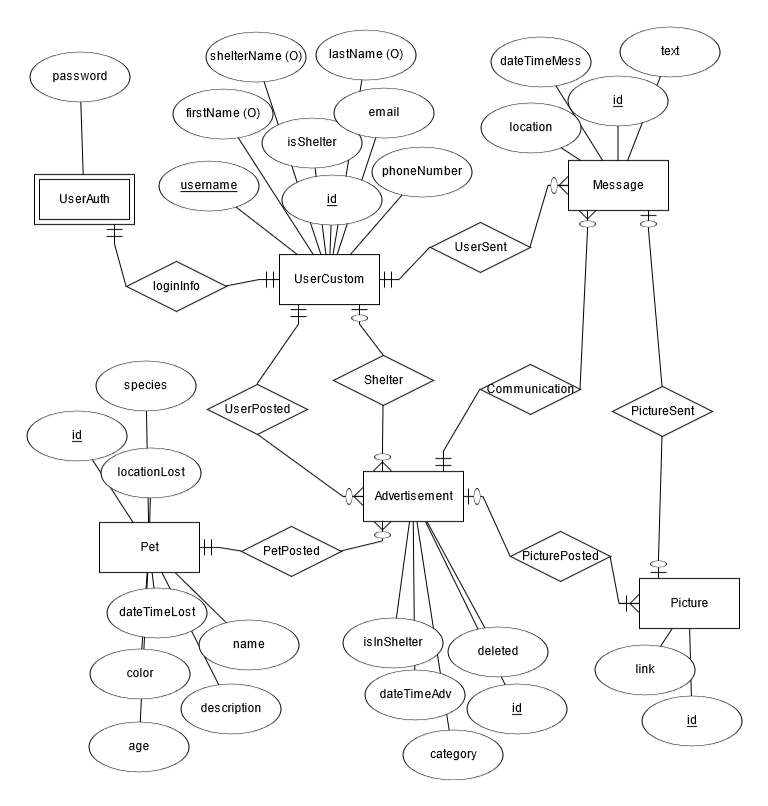
\includegraphics[scale=0.65]{dijagrami/dijagramBaze/ERmodel.PNG} %veličina slike u odnosu na originalnu datoteku i pozicija slike
					\centering
					\caption{E-R dijagram baze podataka}
					\label{fig:erDijagram}
				\end{figure}

			\eject
			
			
		\section{Dijagram razreda}
		
			\textbf{\textit{dio 1. revizije}}\\
			
			Otprilike...
			
			\textbf{\textit{dio 2. revizije}}\\			
			
			Točno...
			
			\eject
		
		\section{Dijagram stanja}
			
			
			\textbf{\textit{dio 2. revizije}}\\
			
			Ne sad...
			
			
			\eject 
		
		\section{Dijagram aktivnosti}
			
			\textbf{\textit{dio 2. revizije}}\\
			
			Ne sad...
			
			\eject
		\section{Dijagram komponenti}
		
			\textbf{\textit{dio 2. revizije}}\\
		
			Ne sad...